\documentclass[10pt,twocolumn]{article}

% use the oxycomps style file
\usepackage{oxycomps}

% usage: \fixme[comments describing issue]{text to be fixed}
% define \fixme as not doing anything special
\newcommand{\fixme}[2][]{#2}
% overwrite it so it shows up as red
\renewcommand{\fixme}[2][]{\textcolor{red}{#2}}
% overwrite it again so related text shows as footnotes
%\renewcommand{\fixme}[2][]{\textcolor{red}{#2\footnote{#1}}}

% read references.bib for the bibtex data
\bibliography{references}

% include metadata in the generated pdf file
\pdfinfo{
    /Title (Combing BLEU with Morphological Segmentation to Evaluate Nahuatl)
    /Author (Ryann Hally)
}

% set the title and author information
\title{Combing BLEU with Morphological Segmentation to Evaluate Nahuatl}
\author{Ryann Hally}
\affiliation{Occidental College}
\email{hally@oxy.edu}

\begin{document}

\maketitle

\section{Introduction}
For my honors project, I created a metric for evaluating machine-produced Nahuatl translations. During my original comprehensive project, I trained a transformer to translate text from Spanish into Nahuatl. Evaluating the accuracy and fluency of the translations produced by the model presented several challenges both in general and for the Nahuatl language specifically, and so for my honors project I decided to adapt an existing metric to the morphology of Nahuatl to see if provided more accurate and useful evaluations.


\section{Problem Context}

Machine translators such as Google Translate \cite{GoogleTranslate} or Deepl \cite{Deepl} are useful and powerful tools, allowing anyone to translate text between languages. A critical part of creating machine translators is accessing them by evaluating the accuracy, fluency, and overall quality of the translations they produce. 

The gold standard of evaluation for machine translators is human feedback. However, this is both expensive and not always possible depending on the resources available to the developers and whether they can find an individual fluent in both the source (starting) language and target (to be translated into) language \cite{BLEUCritique}. A popular alternative to human feedback is automatic evaluation metrics, which take in a generated translation, also called a candidate translation, and output a score through a mathematical formula or machine learning model.

For my original comprehensive project, I trained Google's T5 transformer to translate  text from Spanish into Nahuatl and experimented with different strategies to overcome the insufficient amount of training data in the language pair I had. Understanding how each strategy impacted the quality of the generated translations was thus essential for determining whether each one worked. I was fortunate to be able to incorporate human feedback into my project, but it was not possible for this to be my only source of feedback because of the large number of translations needed to access and compare multiple models. I used three different automatic evaluation metrics to evaluate the models: BLEU \cite{BLEU}, \cite{ChrF}, and \cite{COMETHF}, but soon discovered that these had many shortcomings that reduced the usefulness and accuracy of the feedback they provided.

The shortcoming I will focus on is one with BLEU, as that is the metric I decided to adapt for Nahuatl. BLEU is one of the most, if not the most, commonly used  metrics for machine translation. I will discuss BLEU more in depth in my prior work section, but the concept behind BLEU is to compare candidate translations to reference translations by word. Nahuatl is a polysynthetic language, which means multiple prefixes and suffixies can be added together to form words that would constitute a phrase or sentence in English. For example,  the word \textit{teaxca} translates to "someone's property", with the prefix \textit{-n} meaning "my" and \textit{axca} meaning "property". If a machine translator outputted \textit{naxca} , meaning "my property", it would receive a BLEU score of 0.0 because it is comparing at the word level. Observing this while working on my comprehensive project led me to wonder if using the same formula but at the prefix or suffix level would work better for Nahuatl evaluation, which is the idea of my project.

\section{Technical Background}

Next, I will describe the concepts necessary to understand the project. 

\subsection{Linguistic Terminology}

\subsubsection{Morpheme}

A morpheme is a the smallest unit of language that has independent meaning. In English, "general" and 'ly" are the morphemes that form the word "generally". \cite{Polysynethic}

\subsubsection{Morphological Segmentation}
Morphological segmentation refers to breaking a word down into the morphemes it is composed of. Returning to my previous example, \textit{teaxaca} can be broken into \textit{te-} and \textit{axca}.

\subsection{Evaluation Terminology}
\subsubsection{N-gram}
An n-gram is a sequence of consecutive units, most often characters or words, from a piece of text. \cite{BLEUGoogle}

\subsubsection{Precision}

Precision is the proportion of correctly identified  instances out of all instances. For the evaluation of machine translations, this will refer to the proportion of words, morphemes, or characters in a candidate translation that are seen in the reference translation \cite{GoogleMLEval}. 

\subsubsection{F-Score}

F-score is a combination of precision and recall\cite{GoogleMLEval}, recall being the share of words, morphemes, or characters present in the reference that produced by the candidate \cite{GoogleMLEval}. 


\section{Prior Work}
Next, I will review prior work in automatic evaluation metrics for machine  translations by introducing and discussing several automatic evaluation metrics.

As mentioned previously, BLEU is popular metric for machine translation. It evaluates translations by calculating the precision of overlapping word n-grams between a candidate translation and one or more reference translations, which is then multiplied by a brevity penalty. The brevity penalty means candidate translations shorter than the reference receive a deduction for being shorter. The ensures candidates are not rewarded for leaving out content because they are short but the words they do contain are all or mostly accurate \cite{BLEU}.

BLEU has several flaws or shortcomings. Since it evaluates translations by comparing the word n-gram overlap, it gives candidates translations a high score when they contain all or mostly the same words as the reference. This means translations that convey the same meaning through different words will receive a low BLEU score even if they would be considered an acceptable translations by a human evaluator \cite{BLEUCritique}. Additionally, as explained previously, BLEU presents a particular problem for Nahuatl and polysynthetic languages in general since evaluating by word leads BLEU unable to recognize correct morphemes or parts of words.

Another popular automatic evaluation metric is ChrF. It
scores a translation by calculating the F-score of overlapping character n-grams between the candidate and the reference. Like BLEU, it checks n-gram overlap, but it does so at the character level and combines both precision and recall in a single F-score.

Chrf is considered better suited for the evaluation of polysynthetic languages like Nahuatl but still encounters the same problem of not being able to recognize sematic equivalence. Since Chrf compares by character, partially correct words can be take into account. However, evaluating a word by character as opposed to by morpheme can inflate the score. For example, a word can contains the same letters as the reference word but  none of the same morphemes because ordering is not taken into account, meaning a word that doesn't convey any of same meaning as the reference can still receive a high Chrf score. In terms of the problem of translations with the same meaning but different words, Chrf does not improve on the BLEU's shortcoming in this area because it again is comparing by overlap. 

\section{Methods}

Next, I will explain the methods I used to complete my project and why I chose them. My metric combines BLEU's formula with morphological segmentation. It takes in a translated Nahuatl word or a sentence and its reference translation, splits each into morphemes, and then compares them by morpheme. Thus, my project can be divided into two parts: morpheme segementation and implementation of the BLEU formula. 


\subsection{Morphological Segmentation: Morfessor}

To break Nahuatl candidate and reference translations into morphemes, I used a program called Morfessor \cite{Morfessor}. 

\subsection{Morfessor}

Morfessor refers to a set of models than can be trained to breakdown text into morphemes. It takes in a list of words, and compiles a lexicon, or list of morphemes as it trains on this word list.

I used the Baseline Morfessor model, which is an unsupervised model that learns to segment from a list of words. The baseline model uses a maximum-posterior objective and its prior prioritizes the creation of a lexicon with fewer and shorter morphemes. Its formula is then: 
\begin{figure}
    \centering
    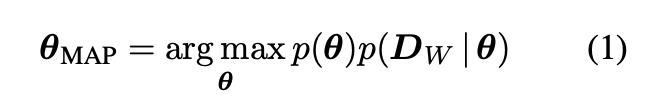
\includegraphics[width=.95\linewidth]{Morfessor1.png}
    \caption{ MAP
    }
    \label{fig:first-page}
\end{figure}

\begin{figure}
    \centering
    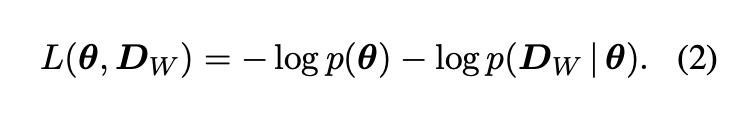
\includegraphics[width=.95\linewidth]{Morfessor2.png}
    \caption{ Cost Function
    }
    \label{fig:first-page}
\end{figure}

\subsection{Training Morfessor}
\subsubsection{Creating a Corpus}
To train Morfessor, I gave it a list of Nahuatl words. The first word list I tried was the Somos-NLP corpus I used for my original project broken into words. However, I wasn't satisfied with the way it was breaking down words after using this word list for training. Additionally, the Morfessor baseline models needs to have seen a word, or to have it in its lexicon, in order to segment it, and this corpus proved  to not be thorough enough for Morfessor to get through any  reference or candidate translations. 
So, I decided to compile a longer word list by scraping words from a website called "Nahuatl Online Dictionary: \cite{NahuatlDictionary}. I used ChatGPT to make a script to iterate through the online dictionary and store each Nahuatl word in a list. I ended up with a list of 100,000+ words.  

\subsection{Training Morfessor}
I trained Morfessor with the list of words from Nahuatl dictionary. It trained for 6 epochs and took approximately 3 minutes to train.

\section{Evaluation Metrics}

To evaluate my project, I compared my metric to human feedback. I did this by compiling a list Spanish sentences and several Nahuatl translations from different translators for each one. I produced rankings of the  translations for each Spanish sentence using my own metric as well as BLEU and ChrF. Then, I asked Professor Sousa to rank the Nahuatl translations. I compared how each of the metrics ranked the translations to Sousa through a statistic called Kendall's Tau. This revealed how my metric evaluated translations in comparison to Sousa, a measure of its alignment with human feedback, as well as how much my metric aligned with human feedback in comparison to BLEU and ChrF.

\section{Example Sentences}
The sentences I translated were selected from the Somos-NLP Hackaton Spanish-Nahuatl parallel corpus I used for my original project \cite{SomosNLP}. This corpus contains Spanish words, phrases, and sentences along with their Nahuatl translations from a variety of sources. I selected several translations from two different sources and made sure they were of varying length as well. I used seven Spanish-Nahuatl translations from \textit{Recetario Nahua}, which is a recipe book that featuring recipes written both Spanish and Nahuatl. I used seven in total from this source: one translation that was one word in both Spanish and Nahuatl, one that was two words in Nahuatl and one in Spanish, two phrases, and three sentences. I used five translations from \textit{Historia de Mexico Narrada en Nahuatl y Español}, three of sentence length and two of paragraph length. 

\section{Translators}
I had four different Spanish-Nahuatl translations translate  each Spanish sentence. They were Google Translate's Spanish-Nahuatl translator which translates specifically into the Eastern Huasteca dialect \cite{GoogleTranslate}, two translators I created in my original project, and the Spanish-Nahuatl translator created by Somos-NLP \cite{SomosNLP} that I used as inspiration for my project.

\section{Gathering Feedback from Professor Sousa}
Professor Sousa is a Latin American studies professor who specializes in the Nahua people and their language. To get her feedback on the translations, I presented her with each Spanish sentence, its Nahuatl reference translation, the four Nahuatl candidate translations and asked her to rank them in comparison to each other.


\section{Kendall's Tau}
Kendall's Tau is a statistic that measures the correlation between two different rankings. In the implementation of Kendall's Tau I used, a coefficient of 1 indicates an exact match while a coefficient of -1 indicates the rankings don't match at all. 

The implementation of Kendall's Tau I used returned a value of NaN if one of the rankings contained all the same value, as in [1,1,1,1]. Since the metrics produced several rankings like this, this meant I was unable to get a coefficient for them. 

\section{Results}

\subsection{Comparison to Professor Sousa's Rankings}

The average Kendall's Tau for the rankings produced by my metric in comparison to the rankings produced by Professor Sousa was .80 for translations from the source \textit{Recetario} and .60 from translations from \textit{Historia de Mexico}.

\subsection{Other Metrics in Comparison to Professor Sousa's Rankings}
\begin{enumerate}
    \item The average Kendall's Tau coefficient for rankings produced by BLEU in comparison to rankings produced by Professor Sousa was .73 for \textit{Recetario Nahua} and .46 for \textit{Historia de Mexico}.
    \item The average Kendall's Tau coefficient for rankings produced by BLEU in comparison to rankings produced by Professor Sousa was.87 for \textit{Recetario Nahua} and .72 for \textit{Historia de Mexico}.
\end{enumerate}

\subsubsection{Impact of Length of Translation}

The average Kendall's Tau coefficient for the rankings produced by my metric in comparison to the rankings produced by Professor Sousa for translations of a length of one to two words was 1, while it earned a coefficient of .67 for translations of one sentence or more.

\section{Results}
\subsection{Comparison to Professor Sousa's Rankings}
My metric earns a Kendall's Tau coefficient of .80 for translations of the source \textit{Recetario Nahua} and .46 for translations from \textit{Historia de Mexico}. Thus, it aligns well with Professor Sousa's rankings for one source but not the other

We can also see that my metric aligns more with Professor's Sousa for translations that consist of one or two words in Spanish and Nahuatl than longer translations. I believe the difference in correlation between the two sources can be explained by this, as the examples from \textit{Recetario Nahua} consist of mostly one word or phrase while the examples from \textit{Historia de Mexico} are all 1-3 sentences long. This means that my metric works better on single word translations than longer translations. 

\subsection{Comparison to Other Rankings}
My metric correlates less with Professor Sousa's rankings than both BLEU and Chrf for \textit{Recetario Nahua} but more than BLEU for \textit{Historia de Mexico}. Thus, it appears to perform about the same as BLEU. This suggests ChrF is the metric most aligned with human feedback for Nahuatl translations and is the most equipped to evaluate the language.

\subsection{Further Discussion}
One shortcoming of my metric and possible explanation why it was not able to improve upon BLEU and ChrF is problems arising from the strategy of morphological segmentation that I chose. Morfessor segments words based on the most common segmentation according to the lexicon balanced with the intent of identifying the smallest morphemes possible. Unfortunately this ensures a reference and a candidate translation can be broken down into morphemes that don't overlap at all just because one letter is different. Returning to my earlier example, if there reference is \textit{naxaca} and the candidate \textit{teaxca}, \textit{naxaca} could be broken into [n] and [axca] while \textit{teaxaca} is broken into [tea] [xca]. This would lead to a score of 0.0, while I intended the score for candidates like this to be 50/100. Using a rule-based segmenter instead of generative probabilistic model would possibly fixed this problem and improved the performance of the metric.

\section{Ethical Considerations}

The principle ethical concern of this project is that is possible for machine translators and evaluation metrics to misrepresent indigenous languages like Nahuatl. Machine translators do not always create accurate or fluent translations yet are often public and widely accessible. Indigenous languages like Nahuatl already face discrimination due to the legacy of European colonization and their status as minority languages in most regions where they are spoken \cite{IndigenousLanguageDeath}. Additionally, they often hold much cultural importance and relevance for Indigenous communities, making this misrepresentation worse \cite{IndigenousLanguages}. Automatic metrics have a slightly lesser but similar ability to misrepresent languages through inaccurate evaluation of translations. 

Thus, it is important to present translators and evaluation metrics as what they are and not confuse them for any authority on the language. They are helpful tools for working with the language, but should not be taken as anything more than that and do not represent the language and serve as any authority on what is correct or incorrect over human speakers. 



\appendix
\section{\\Replication Instructions}
I used Google Colab to train Morfessor, implement the BLEU formula, and obtain the Chrf and BLEU scores of each of my examples translations.

Prerequisites:
\begin{itemize}
    \item Python Version 3.10
    \item Hugging Face account
    \item Hugging Face transformers, datasets, evaluate, and sacreBLEU libraries
    \item SomosNLP Spanish-Nahautl a dataset on Hugging Face
    \item Morfessor Python library
    \item SciPy library
    \item Counter from Collections library

    \end{itemize} 

Training Morfessor
\begin{enumerate}
    \item Import Morfessor
    \item Create iterator for word list
    \item Iterate over word list
    \item Initialize Morfessor baseline model
    \item Load data
    \item Train model with data
    \item Mount Google drive
    \item Save model to Google Drive by writing to file in Google Drive
\end{enumerate}


Implementing BLEU
\begin{enumerate}
    \item Install all libraries
    \item Import Morfessor 
    \item Mount Google Drive
    \item Download saved Morfessor model from Google Drive
    \item Method for calling Morfessor to segment text into morphemes by word
    \item Method for extracting n-grams using Collections library
    \item Method for calculating the precision using morpheme lists
    \item Method for taking in a translation, calling each method and then printing the score
\end{enumerate}


\section{\\Code Architecture Overview}
My code consists of 4 Google Colab notebooks,  one for training Morfessor, one for implementing the metric, and two for calculating Kendall's Tau for each source of example translations

\printbibliography

\end{document}
